\documentclass{beamer}
\usefonttheme[onlymath]{serif}
\usepackage{anyfontsize}

\begin{filecontents*}{\jobname.bib}

  @article{shazeer2017outrageously,
  title={Outrageously large neural networks: The sparsely-gated mixture-of-experts layer},
  author={Shazeer, Noam and others},
  journal={arXiv preprint arXiv:1701.06538},
  year={2017}
}

@article{bahdanau2014neural,
  title={Neural machine translation by jointly learning to align and translate},
  author={Bahdanau, Dzmitry and others},
  journal={arXiv preprint arXiv:1409.0473},
  year={2014}
}

@article{graves2016hybrid,
  title={Hybrid computing using a neural network with dynamic external memory},
  author={Graves, Alex and others},
  journal={Nature},
  volume={538},
  number={7626},
  pages={471--476},
  year={2016},
  publisher={Nature Publishing Group}
}
\end{filecontents*}
\usepackage{natbib}
\usepackage{bibentry}
\bibliographystyle{apalike}

\title{Attention in Neural Networks} % (optional, only for long titles)
%{Deep Learning Book discussion questions}
%\subtitle{}
\author{Erik Ylipää}
\institute{Research Institutes of Sweden}

\renewcommand{\vec}[1]{{\boldsymbol{#1}}}
\newcommand{\tvec}[2]{{\vec{#1}^{(#2)}}}
\newcommand{\svec}[2]{{\vec{#1}_{#2}}}
\newcommand{\stvec}[3]{{\vec{#1}_{#2}^{(#3)}}}


\begin{document}
\nobibliography{\jobname}

\frame{\titlepage}

  \begin{frame}
    \frametitle{Set of vectors}

    \begin{itemize}
    \item
    Imagine we have some set of vectors we want to make predictions based on
  \item
    We'll use the example of natural language in this case. The vectors represents words in a sentence and we would like to predict sentiment of the sentence (does this sentence express a positive or negative opinion).

  \item
    For example, the sentences ``The movie was really good'' or ``I head a great time'' could be represented by the sets
    \begin{itemize}
    \item $\{ \svec{x}{\text{the}}, \svec{x}{\text{movie}}, \svec{x}{\text{was}}, \svec{x}{\text{really}}, \svec{x}{\text{good}} \}$
      \item $\{ \svec{x}{\text{i}}, \svec{x}{\text{had}}, \svec{x}{\text{a}}, \svec{x}{\text{great}}, \svec{x}{\text{time}} \}$
    \end{itemize}
  \item Order is not represented, so the following equality holds
    \begin{itemize}
    \item $\{ \svec{x}{\text{the}}, \svec{x}{\text{movie}}, \svec{x}{\text{was}}, \svec{x}{\text{really}}, \svec{x}{\text{good}} \} = \{ \svec{x}{\text{movie}}, \svec{x}{\text{good}}, \svec{x}{\text{was}}, \svec{x}{\text{the}}, \svec{x}{\text{really}} \}$
    \end{itemize}
    \end{itemize}
  \end{frame}

  \begin{frame}
    \frametitle{Sentiment prediction on word vectors}
    \begin{itemize}
    \item Now imagine we want to predict sentiment based on the words in a sentence
    \item We want to define a function from a set of vectors to a sentiment score (e.g. +1 for positive sentiment, 0 for negative)
      \begin{itemize}

      \item $s(\{ \svec{x}{\text{the}}, \svec{x}{\text{movie}}, \svec{x}{\text{was}}, \svec{x}{\text{really}}, \svec{x}{\text{good}} \}) = 1$
        \item $s(\{ \svec{x}{\text{this}}, \svec{x}{\text{was}}, \svec{x}{\text{the}}, \svec{x}{\text{worst}}, \svec{x}{\text{movie}}, \svec{x}{\text{ever}} \}) = 0$
      \end{itemize}


    \end{itemize}
  \end{frame}

  \begin{frame}
    \frametitle{Sentiment prediction on word vectors using logistic regression}
    \begin{itemize}
          \item A straight forward way of doing this is using logistic regression on a fixed length vector representation of the sentence
      $s = \sigma(W f(\{ \svec{x}{\text{the}}, \svec{x}{\text{movie}}, \svec{x}{\text{was}}, \svec{x}{\text{really}}, \svec{x}{\text{good}} \}) + b), f: \mathbb{X} \rightarrow \mathbb{R}^d$

          \item The free parameters to learn is then $W, b$ and all the vector word representations $\svec{x}{(.)}$.
          \item We need to define the function $f$ which aggregates the set of words into a fixed length vector (since $W$ and $b$ needs to be of fixed size).
          \item One of the simplest choices is just vector sum
            \begin{itemize}
            \item $f(\{ \svec{x}{\text{the}}, \svec{x}{\text{movie}}, \svec{x}{\text{was}}, \svec{x}{\text{really}}, \svec{x}{\text{good}} \}) = \svec{x}{\text{the}}+\svec{x}{\text{movie}}+\svec{x}{\text{was}}+\svec{x}{\text{really}}+\svec{x}{\text{good}}$
            \end{itemize}
    \end{itemize}
    \end{frame}

  \begin{frame}
    \frametitle{Sums of word vectors for NLP}

\begin{columns}
\column{0.65\textwidth}
    \begin{itemize}
    \item We now have a very simple model for sentiment prediction on arbitrarily long sentences:
      \begin{itemize}
      \item $s = \sigma( W (\svec{x}{\text{the}}+\svec{x}{\text{movie}}+\svec{x}{\text{was}}+\svec{x}{\text{really}}+\svec{x}{\text{good}}) + b)$
      \end{itemize}
    \item This model will learn \emph{word polarity}.
      \begin{itemize}
      \item Words which correlates with positive sentiment will tend to point in one direction in the word vector space
      \item words which correlates with negative sentiment will point in the other direction
        \item words with little correlation to sentiment will be orthogonal to this direction
      \end{itemize}
    \end{itemize}
    \column{0.35\textwidth}
        \begin{figure}
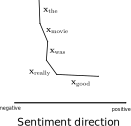
\includegraphics[scale=0.3]{sentiment_analysis_word_vectors}
        \end{figure}
\end{columns}
  \end{frame}
  \begin{frame}
    \frametitle{Issues with sums of word vectors}
    \begin{itemize}
    \item
      Using summation, the sentiment of a sentence is really only determined by sentiment of containing words, not their relation to each other
      \begin{itemize}
      \item “The movie was really great!” and “The movie was not really great!” will likely have almost the same positive sentiment score.
        \item The model can’t modify it’s prediction based on the presence of “not”, since that word vector will not be more strongly correlated with negative sentiment than “great” is with positive
      \end{itemize}
    \item What if we could weight the vectors depending on context?
      \begin{itemize}
      \item The presence of “not” could reduce the value of “great”
      \end{itemize}
    \end{itemize}
  \end{frame}

  \begin{frame}
    \frametitle{Weighted sums}
    \begin{itemize}
    \item Instead of a regular vector sum, we can instead weight each vector
      \begin{itemize}
      \item $f(\{ \svec{x}{\text{the}}, \svec{x}{\text{movie}}, \svec{x}{\text{was}}, \svec{x}{\text{really}}, \svec{x}{\text{good}} \}) = a_{the} \svec{x}{\text{the}}+ a_{movie}\svec{x}{\text{movie}}+ a_{was}\svec{x}{\text{was}}+a_{really}\svec{x}{\text{really}}+a_{great}\svec{x}{\text{good}}$
        \item The $a$'s are scalar and typically constrain the weights so that they are positive and sum to 1, which makes the weighted sum a weighted mean

      \end{itemize}
    \item For this to make sense we would like the weights to actually be computed from the set at hand
    \item If they where fixed for each word, it would be like not having them at all since the word vectors are learned)
    \end{itemize}
  \end{frame}

  \begin{frame}
    \frametitle{Weighted view of the sentence}
    \begin{itemize}
          \item We define a new function, which has the task of producing the weights for our weighted mean
            \begin{itemize}
    \item $g(\{ \svec{x}{\text{the}}, \svec{x}{\text{movie}}, \svec{x}{\text{was}}, \svec{x}{\text{really}}, \svec{x}{\text{good}} \}) = \{ a_{the}, a_{movie}, a_{was}, a_{really}, a_{great} \} $
\end{itemize}

  \item If the weighting function $g$ produces its weights based on the whole context, it's able to change the weight of a word depending on what other words are present in the sentence, e.g. the prescence of the word ``not'':
    \begin{itemize}
    \item {\fontsize{5}{6}\selectfont The} {\fontsize{8}{10}\selectfont movie} {\fontsize{5}{6}\selectfont was} {\fontsize{10}{12}\selectfont really} {\fontsize{40}{48}\selectfont great}!
    \item {\fontsize{5}{6}\selectfont The} {\fontsize{8}{10}\selectfont movie} {\fontsize{5}{6}\selectfont was} {\fontsize{40}{48}\selectfont not} {\fontsize{10}{12}\selectfont really} {\fontsize{6}{7}\selectfont great}!
    \end{itemize}
  \end{itemize}
  \end{frame}

  \begin{frame}
    \frametitle{Attention in neural networks}
    \begin{columns}
      \column{0.3\textwidth}
      \begin{figure}
        \includegraphics[width=\textwidth]{mixture_of_experts}
        \caption{Mixture of Experts}
      \end{figure}
      \column{0.2\textwidth}
      \begin{figure}
        \includegraphics[width=\textwidth]{bahdanu_attention}
        \caption{Information shortcut}
      \end{figure}
      \column{0.5\textwidth}
      \begin{figure}
        \includegraphics[width=\textwidth]{dnc}
        \caption{Memory read and write mechanisms}
      \end{figure}
    \end{columns}
    \vfill
    \tiny \bibentry{shazeer2017outrageously}

    \tiny \bibentry{bahdanau2014neural}

    \tiny \bibentry{graves2016hybrid}
  \end{frame}

  \begin{frame}
    \frametitle{Effect of attention in neural networks}
    \begin{itemize}
    \item Attention in neural networks are often explain in terms of what the mechanism could potentially be used for, like in the example of weighted sums for sentiment analysis
    \item One of the original motivations of attention, as in the mixture of experts examples from the late 1980s, is to isolate parts of the network from change.
    \end{itemize}

  \end{frame}
\begin{frame}
    \frametitle{Attention computational graph example}
      \begin{figure}
        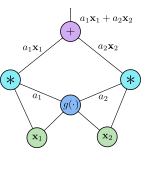
\includegraphics[scale=0.4]{attention_credit_assignment_ops}
        \caption{Simple attention example over two vectors}
      \end{figure}
\end{frame}

\begin{frame}
      \frametitle{Attention computational graph example}
  \begin{figure}
    \includegraphics[scale=0.4]{attention_credit_assignment_ops_error}
        \caption{Example, one vector receives all attention}
      \end{figure}
\end{frame}
\begin{frame}

  \begin{figure}
        \frametitle{Attention computational graph example}
    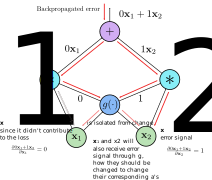
\includegraphics[scale=0.4]{attention_credit_assignment_ops_example}
        \caption{The attention masks the backpropagated error}
      \end{figure}
\end{frame}

\begin{frame}
  \frametitle{Attention variations}
  \begin{itemize}
  \item There are many different ways of computing the attention weights, one can divide them into two main strategies:
    \begin{enumerate}
    \item Fixed attention
    \item Self-attention
    \end{enumerate}
  \item The standard way of making all attention scores be greater than 0 and sum to 1 is to apply the softmax function to them
    \begin{itemize}
    \item $a_i = softmax(\mathbb{A})_i$, where in our example $\mathbb{A} = \{ \alpha_{\text{the}} ,\alpha_{\text{movie}}, \alpha_{\text{was}}, \alpha_{\text{really}}, \alpha_{\text{great}} \}$, the $\alpha$'s are the unnormalized attention scores for each element in the set
    \item Since the softmax is implicit, we will consider the function $g$ to produce unnormalized scores
    \end{itemize}
  \item We'll start looking at fixed attention
  \end{itemize}
\end{frame}
\begin{frame}
  \frametitle{Fixed attention}
  \begin{itemize}
  \item Fixed attention is simple to understand, we learn a function $g$ with parameters $\vec{\theta}$ which takes a single vector as an input. The unnormalized scores are then
    \begin{itemize}
    \item $\mathbb{A} = \{ g(\svec{x}{i}; \vec{\theta}) : \svec{x}{i} \in \mathbb{X} \}$
    \item e.g. $\mathbb{A} = \{ g(\svec{x}{\text{the}}; \vec{\theta}), g(\svec{x}{\text{movie}}; \vec{\theta}), g(\svec{x}{\text{was}}; \vec{\theta}), g(\svec{x}{\text{really}}; \vec{\theta}), g(\svec{x}{\text{good}}; \vec{\theta}) \}$
    \end{itemize}
  \item The function $g(\vec{x}; \theta)$ could be any function, but in neural networks it has typically been either a neural network with a single hidden layer, or just a dot product with the parameter vector $\vec{\theta}$.
    \end{itemize}
    \begin{block}{MLP attention} $g(\vec{x}; W, \vec{b}, \vec{\theta}) = \vec{\theta}^T \sigma({W \vec{x} + \vec{b}}), \vec{x} \in \mathbb{R}^d, W \in \mathbb{R}^{h \times d}, \vec{b} \in \mathbb{R}^h, \vec{\theta} \in \mathbb{R}^h$
    \end{block}
\begin{block}{dot-product attention} $g(\vec{x}; \theta) = \vec{x}^T \vec{\theta}, \vec{x} \in \mathbb{R}^d, \vec{\theta} \in \mathbb{R}^d$
\end{block}

\end{frame}
\begin{frame}
  \frametitle{Fixed attention}
  \begin{block}{dot-product attention} $g(\vec{x}; \theta) = \vec{x}^T \vec{\theta}, \vec{x} \in \mathbb{R}^d, \vec{\theta} \in \mathbb{R}^d$
\end{block}

  \begin{itemize}

  \item We'll focus on dot-product attention. MLP attention is very similar, but input vectors are subjected to an affine transformation before the dot-product attention

  \item I call it fixed, since it will learn a function which gives high score to vectors which have a small angle to its parameter vectors (low angle since both functions use dot products)
  \end{itemize}
\vfill
    \begin{figure}
    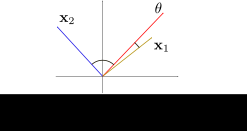
\includegraphics[scale=0.3]{fixed_attention}
    \end{figure}

\end{frame}
\begin{frame}
  \frametitle{Fixed attention}
  \begin{itemize}
  \item This function could help us reweight positive words in the presence of negation
    \begin{itemize}
    \item assign a very high weight by placing the parameter vector close to negating words, leading to a down-weighting of all other words after normalization, especially if the words we would like to be negated are placed in the opposite direction to the $\vec{\theta}$ vector
    \end{itemize}
    \item
      A single fixed attention function can only learn to be senstive along a single direction in input space, the attention becomes very selective
  \end{itemize}
\vfill
    \begin{figure}
    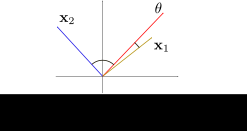
\includegraphics[scale=0.3]{fixed_attention}
    \end{figure}

\end{frame}

\begin{frame}
  \frametitle{Multiple fixed attention functions}
  \begin{itemize}
  \item A solution to the issue of fixed attention selectiveness is to have multiple attention functions $g$

  \item We can think of them each as being attentive of some particular aspect of the input set
    \begin{itemize}
    \item $\mathbb{A}_1 = \{ g_1(\vec{x}) : \vec{x} \in \mathbb{X} \}$, $\mathbb{A}_2 = \{ g_2(\vec{x}) : \vec{x} \in \mathbb{X} \}$

    \item $a_{i,j} = softmax(\mathbb{A}_i)_j$, the softmax function is applied independently to $\mathbb{A}_1$ and $\mathbb{A}_2$
    \end{itemize}

  \item In the end, we can concatenate the outputs of the different attentions
  \end{itemize}
        \begin{align*}
        \svec{v}{1} = \sum_{\svec{x}{i} \in \mathbb{X}} a_{1,i} \svec{x}{i},& \quad \svec{v}{2}=\sum_{\svec{x}{i} \in \mathbb{X}} a_{2,i} \svec{x}{i}\\
        f(\mathbb{X}) =& \begin{bmatrix} \svec{v}{1} \\ \svec{v}{2} \end{bmatrix}
      \end{align*}

\end{frame}
\begin{frame}
  \frametitle{Multiple fixed attention functions}
  \begin{itemize}
  \item In the case of dot-product attention, this would look (almost) like
    \begin{align*}
      \svec{v}{1} = \sum_{\svec{x}{i} \in \mathbb{X}} g_1(\svec{x}{i}) \svec{x}{i},
      \quad \svec{v}{2}=\sum_{\svec{x}{i} \in \mathbb{X}} g_2(\svec{x}{i}) \svec{x}{i},
      \quad f(\mathbb{X}) =& \begin{bmatrix} \svec{v}{1} \\ \svec{v}{2} \end{bmatrix}
    \end{align*}

  \item I say almost since we're omitting the normalization of the outputs of the  $g$'s through application of softmax

  \item We could rewrite this without the g's into
    \begin{align*}
      \svec{v}{1} = \sum_{\svec{x}{i} \in \mathbb{X}} (\svec{x}{i}^T\svec{\theta}{1}) \svec{x}{i},
      \quad \svec{v}{2}=\sum_{\svec{x}{i} \in \mathbb{X}} (\svec{x}{i}^T\svec{\theta}{2}) \svec{x}{i},
      \quad f(\mathbb{X}) =& \begin{bmatrix} \svec{v}{1} \\ \svec{v}{2} \end{bmatrix}
    \end{align*}
  \item The difference between $g_1$ and $g_2$ is really the parameter vectors $\svec{\theta}{1}$ and $\svec{\theta}{2}$

  \end{itemize}

\end{frame}
\begin{frame}
  \frametitle{Multiple fixed attention functions}
  \begin{itemize}
    \item The difference between $g_1$ and $g_2$ is really the parameter vectors $\svec{\theta}{1}$ and $\svec{\theta}{2}$

    \item Instead of considering the attention score functions as being different functions parameterized by $\vec{\theta}$'s, we can think of it as a single function which takes two arguments:
      \[ g(\vec{q}, \vec{k}) = \vec{q}^T \vec{k} \]

    \item Where the vector $\vec{q}$ is the \emph{query}, the vector we wish to calculate attention for and $\vec{k}$ is the \emph{key}, the vector which determines the attention score.
    \item In fixed attention, each attention function is now replaced by a different key vector.
  \end{itemize}

\end{frame}

\begin{frame}
  \frametitle{General attention framework}
  \begin{itemize}
  \item Up until now we have assumed that the vectors we perform the weighted sum on are the same as those used as \emph{queries}. This doesn't have to be the case. A generalized attention function is typically one which takes three arguments

    \[ f(\mathbb{Q}, \mathbb{K}, \mathbb{V}) \]

   {\footnotesize
  \item[$\mathbb{Q}$] The query set, each element of this set has a
    corresponding element in $\mathbb{V}$. We can think of this as how
    each element of our input set \emph{looks} to the attention
    function. Another way to think about it is as an indexing set for
    $\mathbb{V}$.
  \item[$\mathbb{K}$] The key set. We can think of this as being
    \emph{template} vectors the attention function uses to determine
    what to attend to. Each element of $\mathbb{K}$ will be used to
    produce one weighted sum of the vectors in $\mathbb{V}$, so the
    output of our attention will have as many vectors as there are
    elements of $\mathbb{K}$.
     \item[$\mathbb{V}$] The value set. These are the vectors we
       perform the weighted sum on using the attention scores
       calculated based on the queries and keys.
}
    \end{itemize}


\end{frame}

% \begin{frame}
% \frametitle{General attention framework}
%   \begin{itemize}
%   \item Up until now we have assumed that the vectors we perform the weighted sum on are the same as those used as \emph{queries}. This doesn't have to be the case. A generalized attention function is typically one which takes three arguments
%     \[ f(\mathbb{Q}, \mathbb{K}, \mathbb{V}) \]
%     \begin{describe}
%     \item[$\mathbb{Q}$] The query set, each element of this set has a corresponding element in $\mathbb{V}$
%     \item[$\mathbb{K}$] The key set. Each element here will produce one weighted vector using dot-product attention with the elements in the query set to weight all elements in the value set
%       \item[$\mathbb{V}$] The value set. These are the vectors we perform the weighted sum on
%       \end{describe}

%    \end{itemize}

% \end{frame}

\end{document}
